\chapter{Signalweiterleitung im biologischen Neuron}\label{ch:neuron}

Eingehende Signale empfängt eine Nervenzelle über seine \textbf{Dendriten}: Baumförmige Fortsätze, die um den Zellkörper - das \textbf{Soma} - herum gelagert sind.
Sie fungieren \textit{postsynaptisch} und empfangen über \textbf{Rezeptoren} afferente Signale in Form von \textbf{Neurotransmittern} (siehe Abbildung~\ref{fig:neuron}).

\begin{figure}[h]
 \begin{center}
 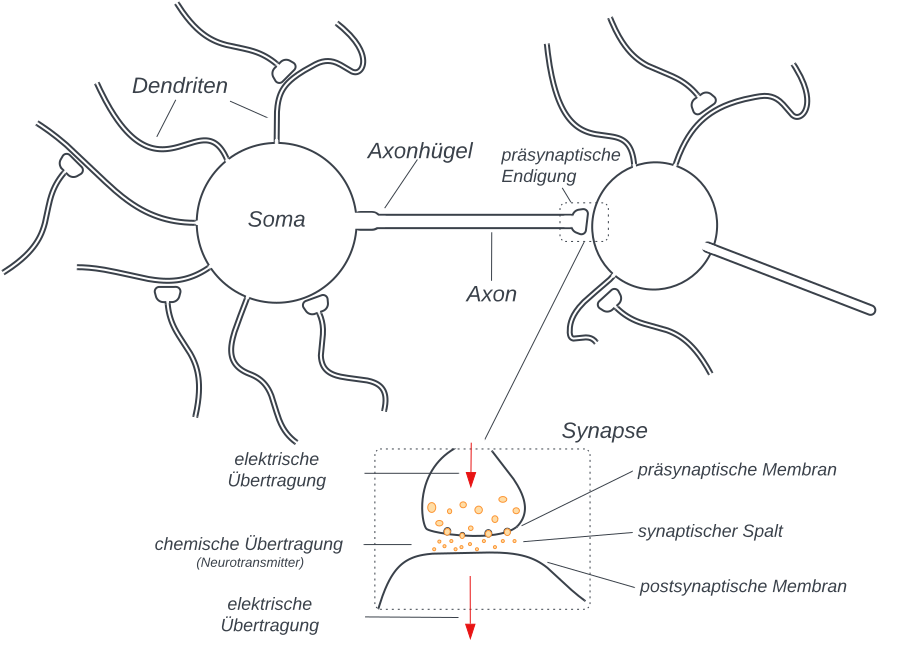
\includegraphics[
  width=16cm,
  keepaspectratio,
 ]{chapters/2. Das Neuron/images/nervenzelle}
 \caption{Schematische Darstellung einer Nervenzelle. (Quelle: in Anlehnung an~\cite[43, Tafel 2.1]{SD07})}
 \label{fig:neuron}
 \end{center}
 \small{
 Die Dendriten leiten afferente Signale zum Soma, dem Zellkörper. Das Axon leitet ein efferentes (``efferre``
  (lat.): hinaustragen, mitnehmen) Nervensignal über präsynaptische Endigungen (auch ``Axonterminale``) an (häufig weit entfernte) Effektoren wie Muskeln, Drüsen oder nachgeschaltete Neuronen weiter.}
\end{figure}

Dendriten leiten die Signale weiter an das Soma, in dem sich, durch die \textbf{Neuronenmembran} von der Umgebung getrennt, \textbf{Zytosol} befindet: Eine salzige, wässrige Flüssigkeit mit einem hohen Anteil von Kalium.

Ob das Neuron Signale weiterleitet, entscheidet sich in der Nähe des \textbf{Axonhügels}: Hier entspringt das \textbf{Axon}, das in einer ``salzigen extrazellulären Flüssigkeit mit hoher Leitfähigkeit`` liegt~\cite[61]{BCP18}.
Eine Depolarisation der Membran an dieser Stelle kann ein \textbf{Aktionspotenzial} auslösen (vgl.~\cite[142 f.]{BCP18}).


\section{Ionenkonzentrationen und Membranspannungen}\label{sec-ionenkonzentrationen}

Ein Neuron weist \textit{in Ruhe} eine ungleiche Ionenverteilung zwischen der durch die Zellmembran getrennten \textbf{intrazellulären Flüssigkeit} (das Zytosol, im folgenden auch IZF) und der \textbf{extrazellulären Flüssigkeit} (im folgenden EZF) auf.
In der IZF befinden sich mehr positiv geladene Natrium-Ionen ($Na^+$), und in der EZF mehr positiv geladene Kalium- und Calcium-Ionen ($K^+$ und $Ca^{2+}$) sowie mehr negativ geladene Chlorid-Ionen ($Cl^-$). Die Membran selber ist mit \textbf{Ionenkanälen} durchsetzt, von denen viele \textbf{selektiv permeabel} sind.\\

{\renewcommand{\arraystretch}{1.5}%
\begin{table} %[hbtp]
 \centering
 \begin{tabular}{l | c | c | c }
  \textbf{Ion} & \textbf{Konzentration EZF (mmol/l)} & \textbf{Konzentration IZF (mmol/l)} & \textbf{Verhältnis} \\
  \hline
  $K^+$      & 5 & 100 & 1 : 20 \\
  $Na^+$     & 150 & 15 & 10:1 \\
  $Ca^{2+}$  & 2 & 0,0002 & 10000 : 1 \\
  $Cl^-$     & 150 & 13 & 11,5 : 1 \\
 \end{tabular}
 \caption{Ionenkonzentration eines Neurons in Ruhe (Quelle: ~\cite[75, Abb. 3.15]{BCP18})}
 \label{tab:ionenkonzentration}
\end{table}

Wenn kein \textbf{postsynaptisches Potenzial} (PSP) wirkt und das Neuron selber keinen Impuls abgibt, liegt das Ruhepotenzial $V_r$ der Zelle zwischen $-70 mV$ und $-90 mV$: Das Zytosol weist entlang der Membranoberfläche in der IZF eine negative Ladung auf.
Diese \textbf{Membranspannung} $V_m$ wird durch eine ungleiche Ionenverteilung bewirkt, verursacht durch die Ladung der Teilchen in der IZF und EZF in Membrannähe (siehe Abbildung~\ref{fig:ionenverteilung}).\\


\begin{figure}[htpb]
 \begin{center}
 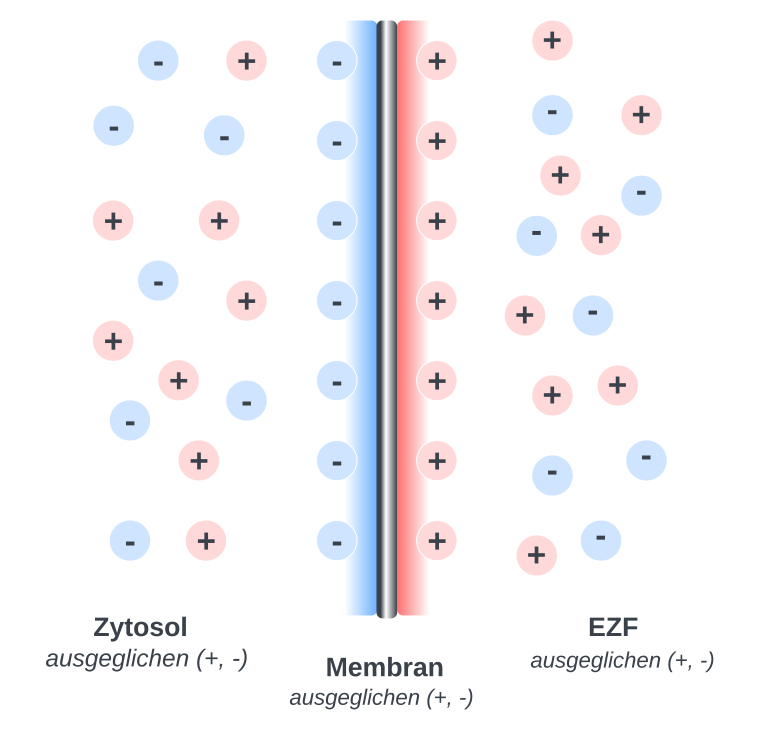
\includegraphics[
  width=8cm,
  keepaspectratio,
 ]{chapters/2. Das Neuron/images/ionenverteilung}
 \caption{Ionenverteilung im Zytosol und der EZF. (Quelle: in Anlehnung an~\cite[72, Abb. 3.13]{BCP18})}
 \label{fig:ionenverteilung}
 \end{center}
 \small{
  Aufgrund der elektrostatischen Anziehungskraft ziehen sich Anionen (neg. geladen) und Kationen (pos. geladen) in der Nähe der Membran gegenseitig an, es kommt zu einer negativen Spannung in Membrannähe (zwischen $-70 mV$ und $-90 mV$ in Ruhe). Dadurch ist die negative Ladung nicht gleichmässig im Zytosol verteilt. \textit{Bear et al.} weisen darauf hin, dass trotzdem der größte Teil des Zytosols und der EZF elektrisch neutral ist (vgl.~\cite[72, Abb. 3.13]{BCP18})}
 }
\end{figure}

In Ruhe ist die Leitfähigkeit der Membran für $Na^+$ gering, für $K^+$ hingegen hoch (vgl.~\cite[44]{SD07}).
$K^+$-Ionen folgen ihrem \textbf{Konzentrationsgradienten} und gelangen über die Ionenkanäle in die EZF, bis die \textbf{Potenzialdifferenz} entlang der Neuronenmembran ausströmende $K^+$-Ionen zurückhält: Wenn diese Differenz den Konzentrationsgradienten für $K^+$ kompensiert, ist das \textbf{Gleichgewichtspotenzial} erreicht, und es findet keine Nettoionenbewegung statt\footnote{
 vgl. ~\cite[72]{BCP18}. \textit{Kandel et al.} schreiben hierzu:
 ``the equilibrium potential of any ion that is present on both sides of a membrane permeable to that ion``~\cite[130]{KSJ+13}
}.


\section{Das Aktionspotenzial}\label{sec:aktionspotenzial}

In Ruhe ist die Ladung in Membrannähe in der IZF negativ, in der EZF positiv.
Durch eine schnelle Umkehrung dieser Verhältnisse ist eine Nervenzelle dazu in der Lage, ein Signal auszulösen (vgl.~\cite[86]{BCP18}).
Hierzu bedarf es eines \textbf{Aktionspotenzials}, das durch Ionenbewegungen entsteht. Die Ionenbewegungen selber sind auf die Änderung des Membranpotenzials zurückzuführen, wodurch ein Öffnen oder Schliessen von ionenspezifischen Kanälen verursacht wird (vgl.~\cite[96]{BCP18}).

 \textit{Kandel et al.} führen 4 wichtige Eigenschaften des Aktionspotenzials auf (vgl.~\cite[148 f.]{KSJ+13}):
\begin{enumerate}
 \item Es gibt einen \textbf{Schwellenwert} für die Auslösung des Potenzials.
 \item Das Aktionspotenzial ist ein \textbf{Alles-oder-Nichts} Ereignis.
 \item Das Aktionspotenzial wird ohne Verlust weitergeleitet.
 \item Nach dem Auslösen des Aktionspotenzial kommt es zu einer \textbf{Refraktärzeit}, in der zunächst kein weiteres Aktionspotenzial ausgelöst werden kann (\textbf{absolute Refraktärzeit}). Bevor $V_r$ wieder erreicht ist, wird für eine kurze Dauer ein stärkeres Signal benötigt, um das Aktionspotenzial erneut auszulösen (\textbf{relative Refraktärzeit}).
\end{enumerate}


\subsection{Auslösung eines Aktionspotenzials}

\begin{figure}[h]
 \centering
 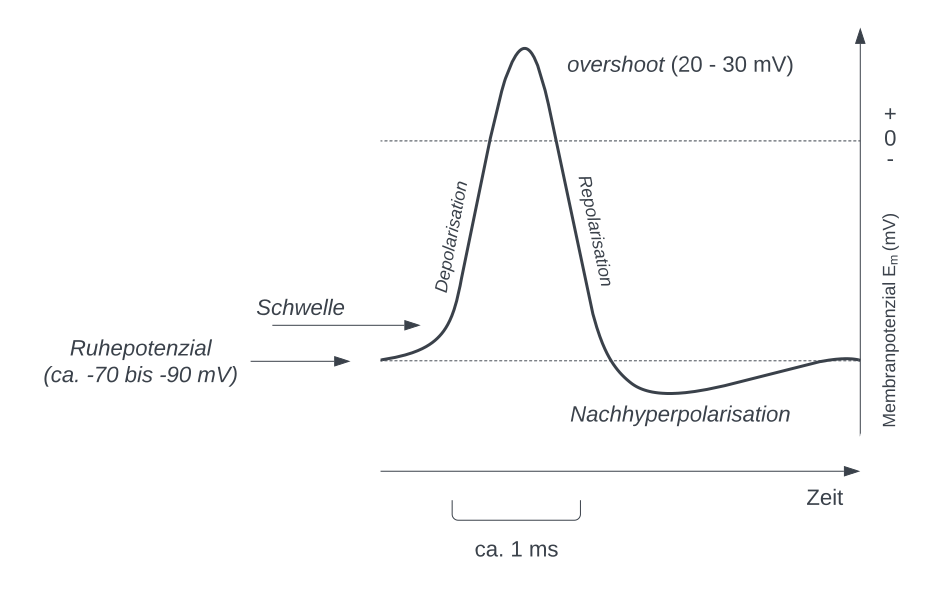
\includegraphics[
  width=12cm,
  keepaspectratio,
 ]{chapters/2. Das Neuron/images/aktionspotenzial}
 \caption{Aktionspotenzial. (Quelle: in Anlehnung an~\cite[47, Tafel 2.3]{SD07})}
 \label{fig:aktionspotenzial}
 \end{figure}


Die \textbf{Initiationszone} des Aktionspotenzials ist der Axonhügel. Hier findet sich eine besonders dichte Anhäufung von spannungsabhängigen $Na^+$-Kanälen, deren Aktivierungskurve um ca. $10 mV$ zu den negativen Membranpotenzialen verschoben ist, was die Initiierung des Signals begünstigt (vgl. ~\cite[77]{Jon19}).

Damit ein Aktionspotenzial ausgelöst werden kann, muss die Membran nahe der Initiationszone über ihren \textbf{Schwellenwert} \footnote{
 ``das kritische Niveau der Depolarisation, das überschritten werden muss, um ein Aktionspotenzial auszulösen``~\cite[88]{BCP18} oder auch ``Erregungsschwelle``~\cite[69]{FE19}.
} $V_t$ ( > $V_r$ ) depolarisiert werden (vgl.~\cite[111]{BCP18}). Erst wenn dieser Schwellenwert übertroffen wird, ``feuert`` das Neuron: Aktionspotenziale funktionieren deshalb nach dem \textbf{Alles-oder-Nichts-Prinzip} (vgl.~\cite[157]{KSJ+13}).

\subsection{Signalweiterleitung über das Axon}

Kurz nach der Aktionspotenzialbildung befinden sich daran beteiligte Membrane in der Refraktärphase, ihre $Na^+$-Kanäle sind inaktiviert. 
Somit pflanzt sich das Aktionspotenzial nur in eine Richtung fort\footnote{\textit{orthodrome} Fortleitung.
  \textit{Bear et al.} verweisen auf \textit{antidrome} Fortleitung (entgegengesetzte Verlaufsrichtung), die in Experimenten ausgelöst werden kann~\cite[106]{BCP18}
} (vgl.~\cite[106]{BCP18}).
Die Fortleitung geschieht in Richtung der Axonterminal, wo sich die präsynaptischen Endigungen befinden und das elektrische Signal in chemische Signale umgewandelt werden (siehe Abbildung~\ref{fig:neuron}). Die durch das Aktionspotenzial ausgelöste Depolarisation der Membran an den Axonterminalen bewirkt eine Öffnung spannungsgeladener Calcium-Kanäle (vgl.~\cite[184]{KSJ+13}). Calcium-Ionen strömen in das Innere der Zelle und lösen die Exozytose von \textbf{synaptischen Vesikeln} aus, kleine, mit einer Membran von der IZF getrennte Strukturen von etwa $50 nm$ Durchmesser, die mit Neurotransmittern gefüllt sind (vgl.~\cite[1000]{BCP18}).

Rezeptoren an den postsynaptischen Endigungen der Folgezelle wandeln diese Botenstoffe in hemmende oder erregende Signale um, die dann nach dem \textbf{Alles-oder-Nichts-Prinzip} erneut integriert werden.


